Geographical data are typically visualized using various information layers
that are displayed over a map. Interactive exploration by zooming and
panning actions needs real-time re-calculation. A common operation in
calculating with multidimensional data is the computation of aggregates.
For layers containing aggregated information derived from voluminous data
sets (see for example Figure~\ref{fig:NL-screenshot}), such real-time
exploration is impossible using standard database technology. Calculations
require too much time.

The University of Twente has developed \emph{``Stairwalker''}: database
technology that accurately aggregates data so that they can geographically
be explored in real-time. The technology is a plug-in to common open
source technology.

Its core is the \emph{pre-aggregate index}: a database index that cleverly
pre-calculates aggregation values such that it can obtain exact aggregation
results from voluminous data with high performance.  A fast calculation
allows to fully recalculate the result for even the slightest movement of
the map, such as a panning or zooming action, without loss of accuracy.
Thanks to this indexing mechanism, we can provide a scalable real-time
calculation: an order of magnitude larger dataset requires only one
additional aggregation level.

In geo data visualization, the ability to quickly develop new information
layers is important. Although many solutions exist, there is a niche: the
combination of visualizing aggregation information, interactive data
exploration in real-time, Big Data, calculating exact numbers instead of
approximations, and doing so with common open source technology. Our
technology for the first time integrates all these features.

\begin{figure}[t]
\centering
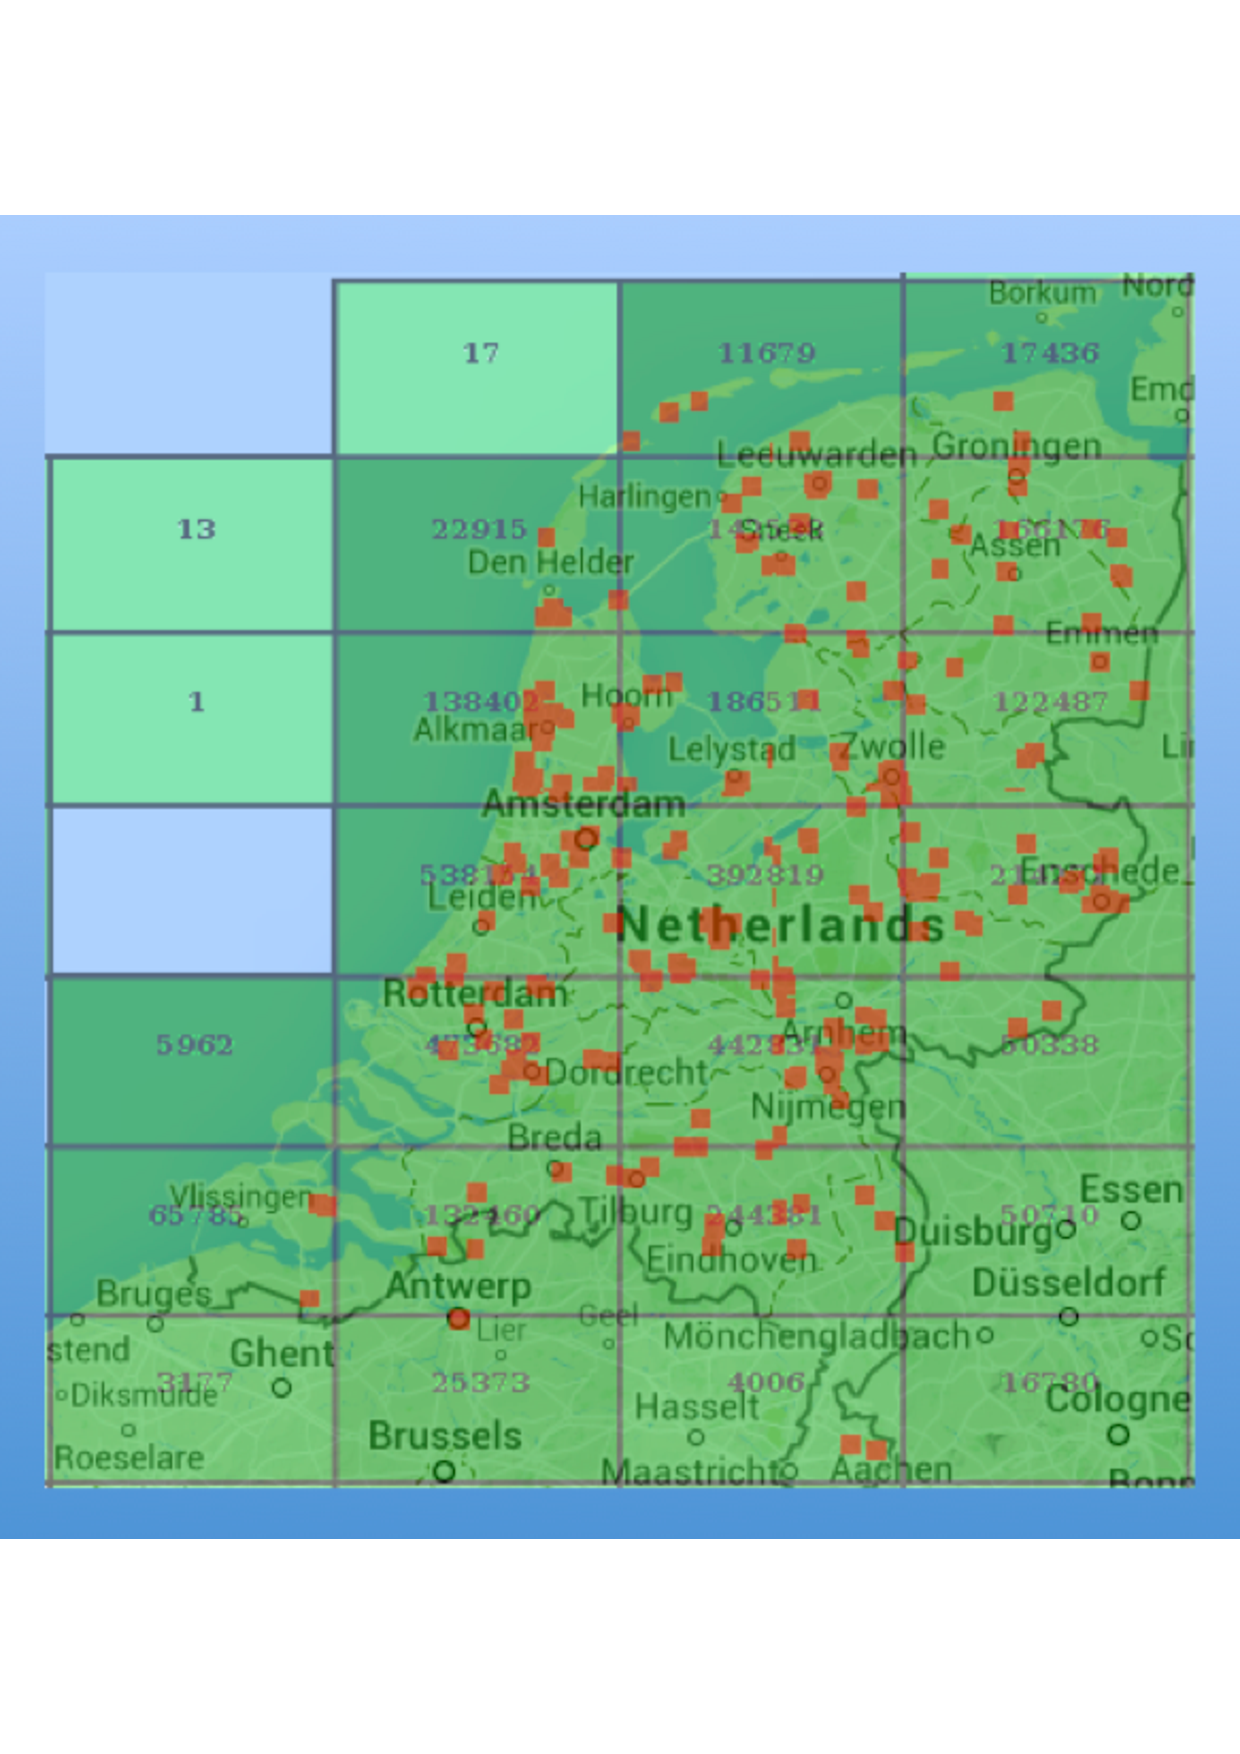
\includegraphics[height=4in]{Figures/NL-screenshot.pdf}
\caption{Twitter hotspot detection in The Netherlands, using a coarse grid.
The numbers inside the grid cells on the map require an aggregation
operation in the database.}
\label{fig:NL-screenshot}
\end{figure}


Our research partners are the companies Arcadis and Nspyre. They both have
struggled with this combination of requirements in many of their projects.
Our database index technology is not specific to geographical data. It can
be used with all types of multidimensional data. Visualization in business
intelligence or eScience can also benefit from it.

\begin{figure}[t]
\centering
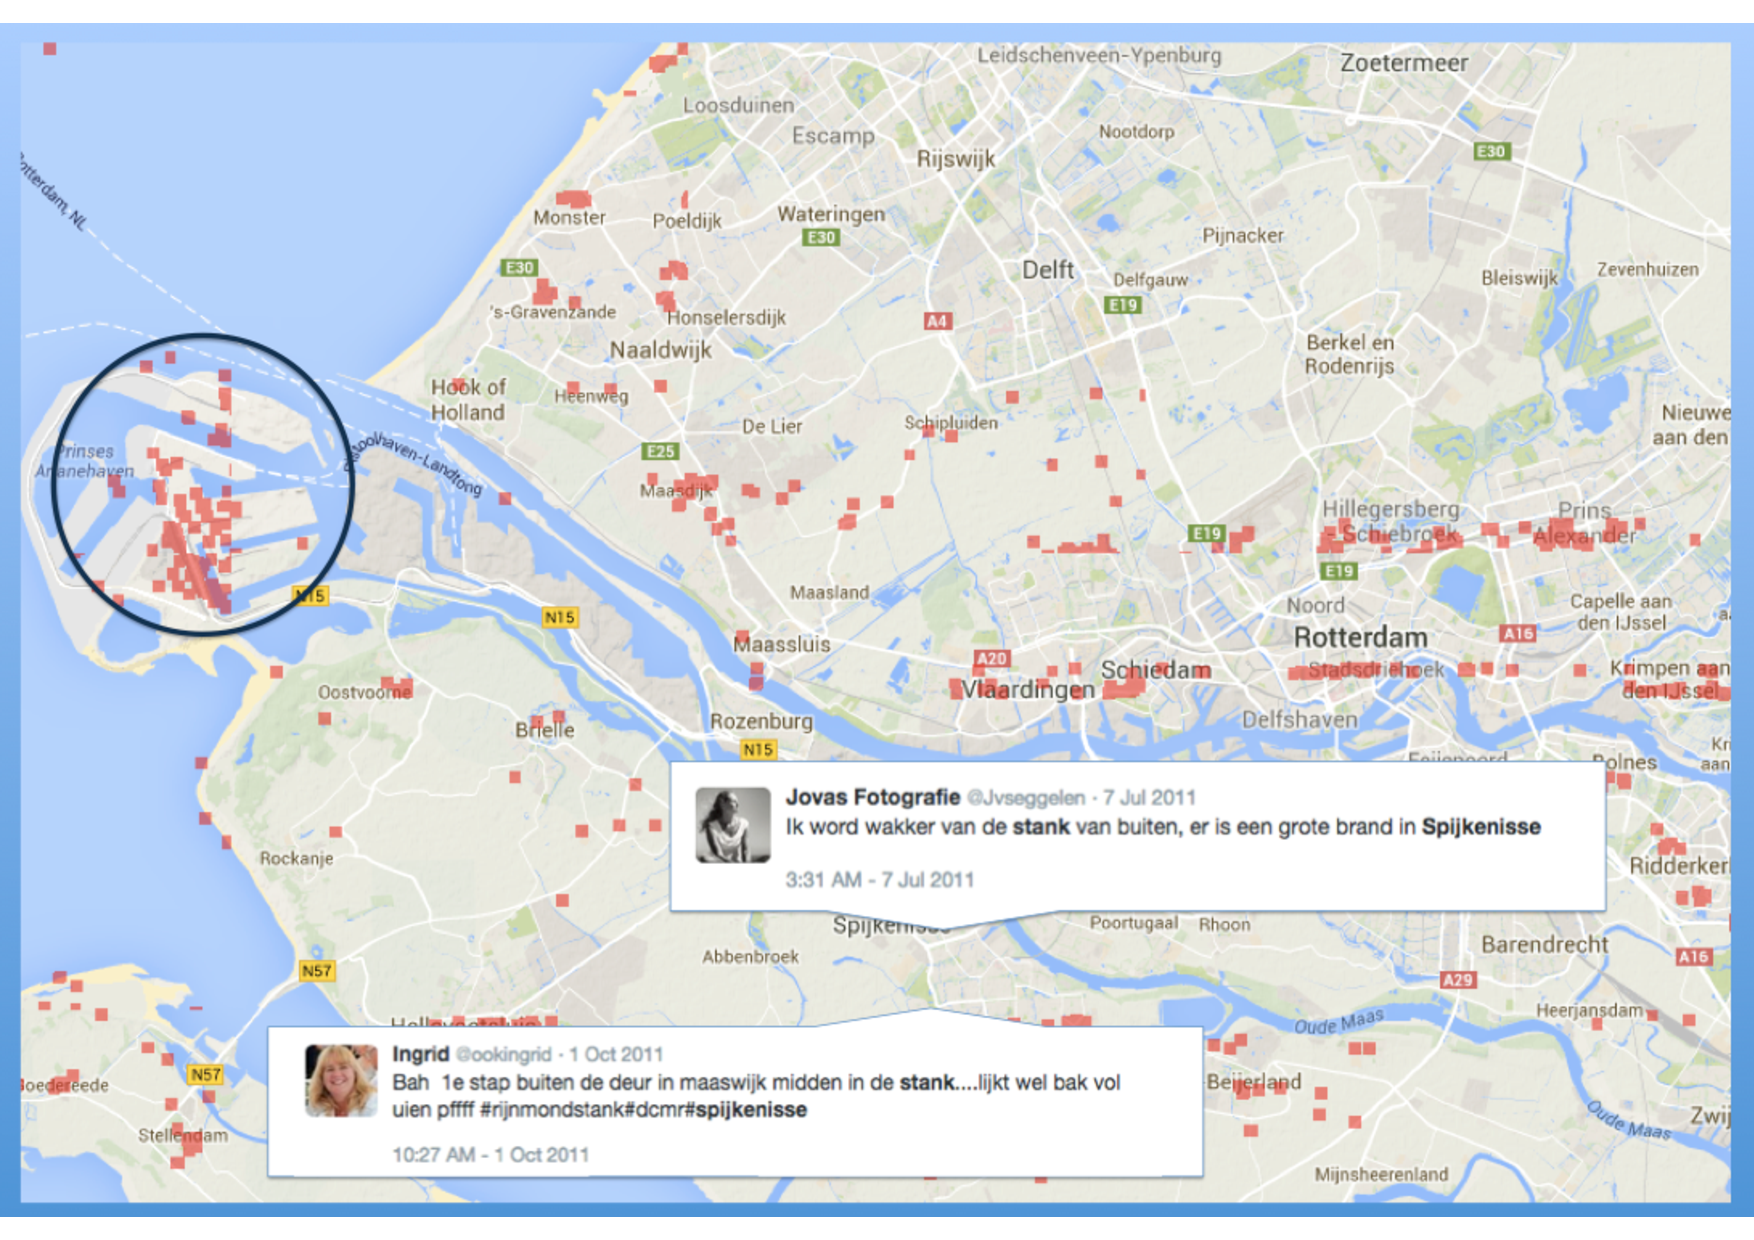
\includegraphics[width=4in]{Figures/DCMR-screenshot.pdf}
\caption{Tweets about excessive smells in the vicinity of the Rotterdam
harbor}
\label{fig:DCMR-screenshot}
\end{figure}

\paragraph{Nice to know}
The company Arcadis developed an application for the DCMR Milieudienst
Rijnmond based on the Stairwalk technology to investigate whether people
send tweets about unpleasant odors as a possible signal of danger (see
Figure~\ref{fig:DCMR-screenshot}). This turns out not to be the case,
probably because people think that nobody reads the tweets anyway. But if
people have the idea that their complaining tweets are read, then tweets
might be much more convenient than the reporting of unpleasant odors by
telephone.

\paragraph{This manual}

This manual explains how to use Stairwalker.  We first explain in
Section~\ref{sec:setup} how to install the required components in order to
have a basic running system.  We then explain in
Section~\ref{sec:deployment} how to add databases and different kinds of
datatypes to Geoserver, an open source server for sharing geospatial
data.\footnote{\url{http://geoserver.org}} It is explained how to show and
customize layers and views, but also how to adjust the system, for example,
how to add dimensions or use different dimension types such as median.
Finally, Section~\ref{sec:development} explains how to extend the system.

\paragraph{Acknowledgements}

This publication was supported by the Dutch national program COMMIT/.
